\chapter{Results}

\begin{center}
    \textit{This chapter presents the outcomes of the project, including the functionality and performance of the developed application. It highlights the achieved results in relation to the project goals and requirements.}
\end{center}

\section{Overview of Delivered Product}
The application was developed as an open-source project with the intention that the code can be reused, maintained, and extended by others. All components are built using open and freely available technologies, ensuring that the system can be installed on local hardware without the need for licensed software or cloud-based services. This aligns with the requirement that all processing should be performed locally, using common hardware such as a webcam connected to a local machine running either Windows or Ubuntu. \\

The project follows clear coding standards and development best practices, making the code easy to understand and modify. All functionality is well documented, enabling future developers to build upon the existing solution. For example, to support new chess variants, integrate additional hardware, or improve the recognition models. To support future development and accessibility, the source code is published in a public Git repository without restrictions on reuse or adaptation. \\

The application itself is a local, camera-based system for digitalizing over-the-board chess games in real-time. It detects piece movements on a physical chessboard using image recognition and converts the game into a \gls{pgn} file, which can be viewed or analyzed digitally. The system operates entirely on local hardware, with a front-end interface that allows users to follow games live and a back-end that manages board recognition and game logic. The application is designed to be low-cost, open-source, and easy to maintain, with extensibility in mind for future features. \\

The delivered product refers to the final version of the application submitted at the conclusion of this Bachelor’s thesis. The application was developed at the request of the product owner and based on the requirements provided. The initial description served as a general concept rather than a detailed specification, which meant that decisions regarding design, architecture, and technology were left to the development team. Throughout the development process, ideas and design choices were discussed with the product owner and approved during regular meetings.

\section{Detection Performance Models}
As a baseline for evaluating detection performance, results from ChessCam repository were first considered \cite{github:chesscam}. These metrics represent the upper-bound performance of the models under ideal conditions. \\

Figure~\ref{fig:chesscam-piece-metrics} illustrates the performance of the piece detection model, which demonstrates consistently high precision and recall throughout training. Both metrics rapidly converge above 0.95, indicating stable and reliable detection \cite{wandb:piece-detection}. In contrast, Figure~\ref{fig:chesscam-xcorners-metrics} presents the results for xcorners detection, showing moderately lower performance. Precision and recall improve steadily over time and stabilize at approximately 0.8 and 0.75, respectively \cite{wandb:xcorner-detection}. \\

\begin{figure}[H]
\centering
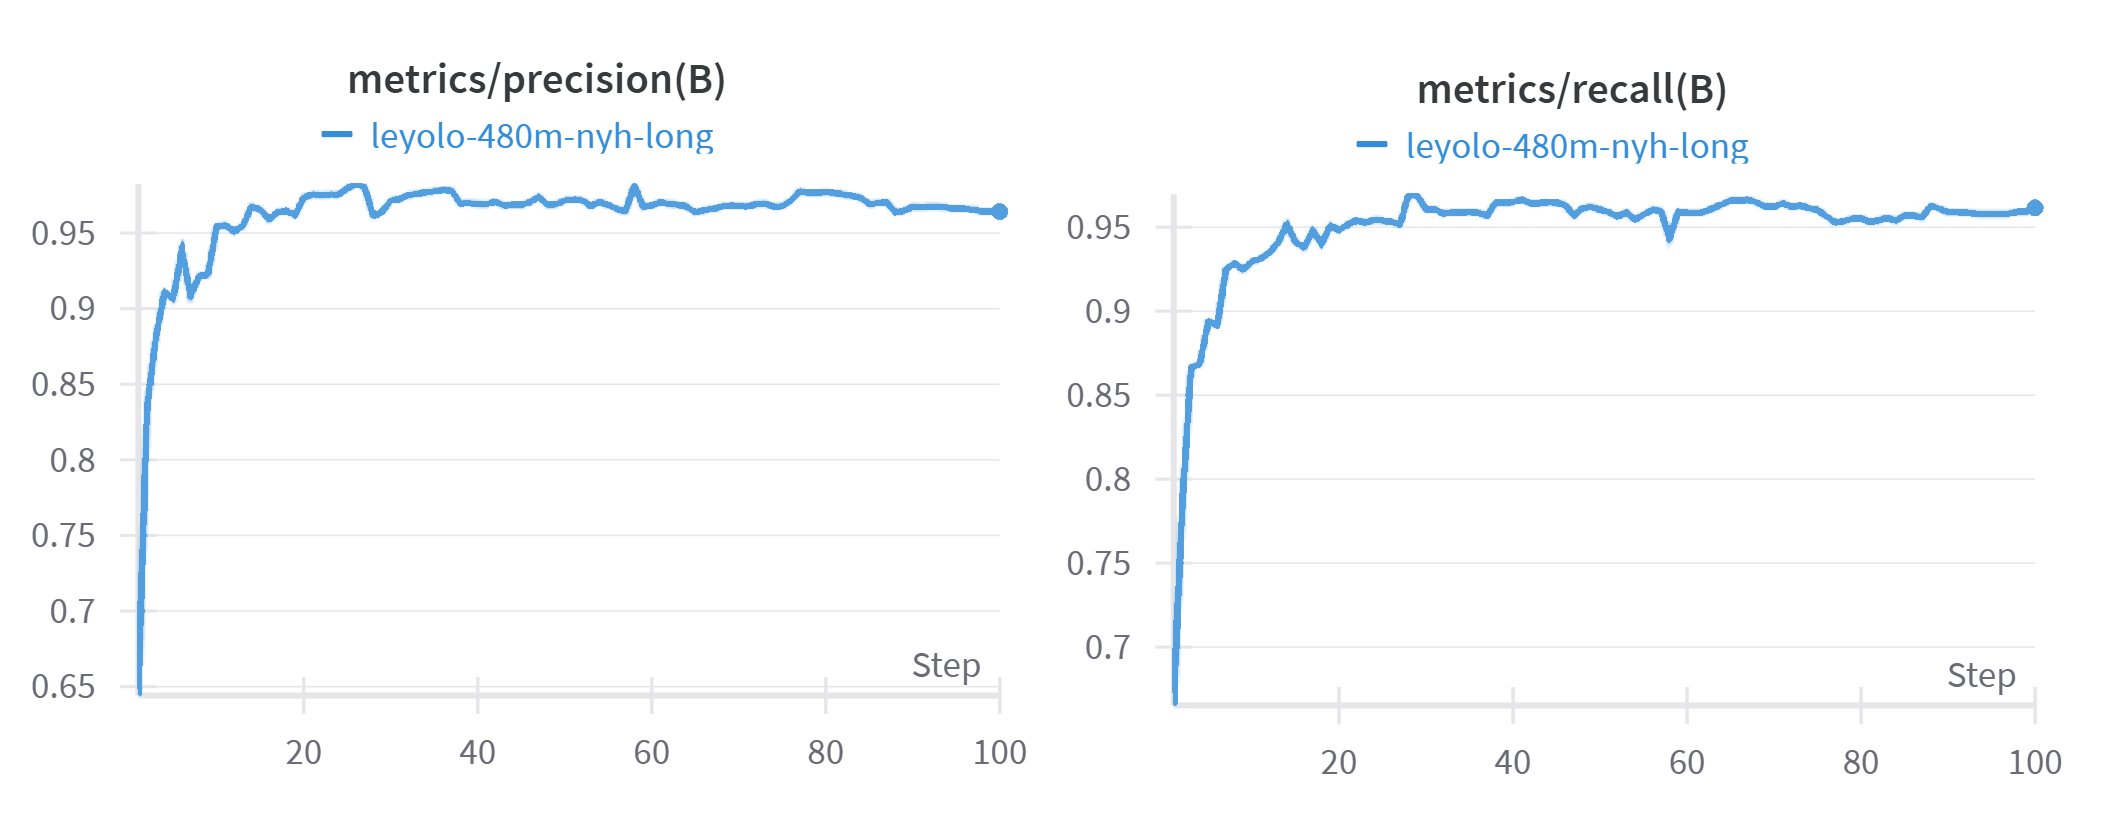
\includegraphics[width=\textwidth]{figures/results/machine-learning/piece-metrics.png}
\caption{Performance metrics for piece detection from ChessCam repository \cite{wandb:piece-detection}.}
\label{fig:chesscam-piece-metrics}
\end{figure}

\begin{figure}[H]
\centering
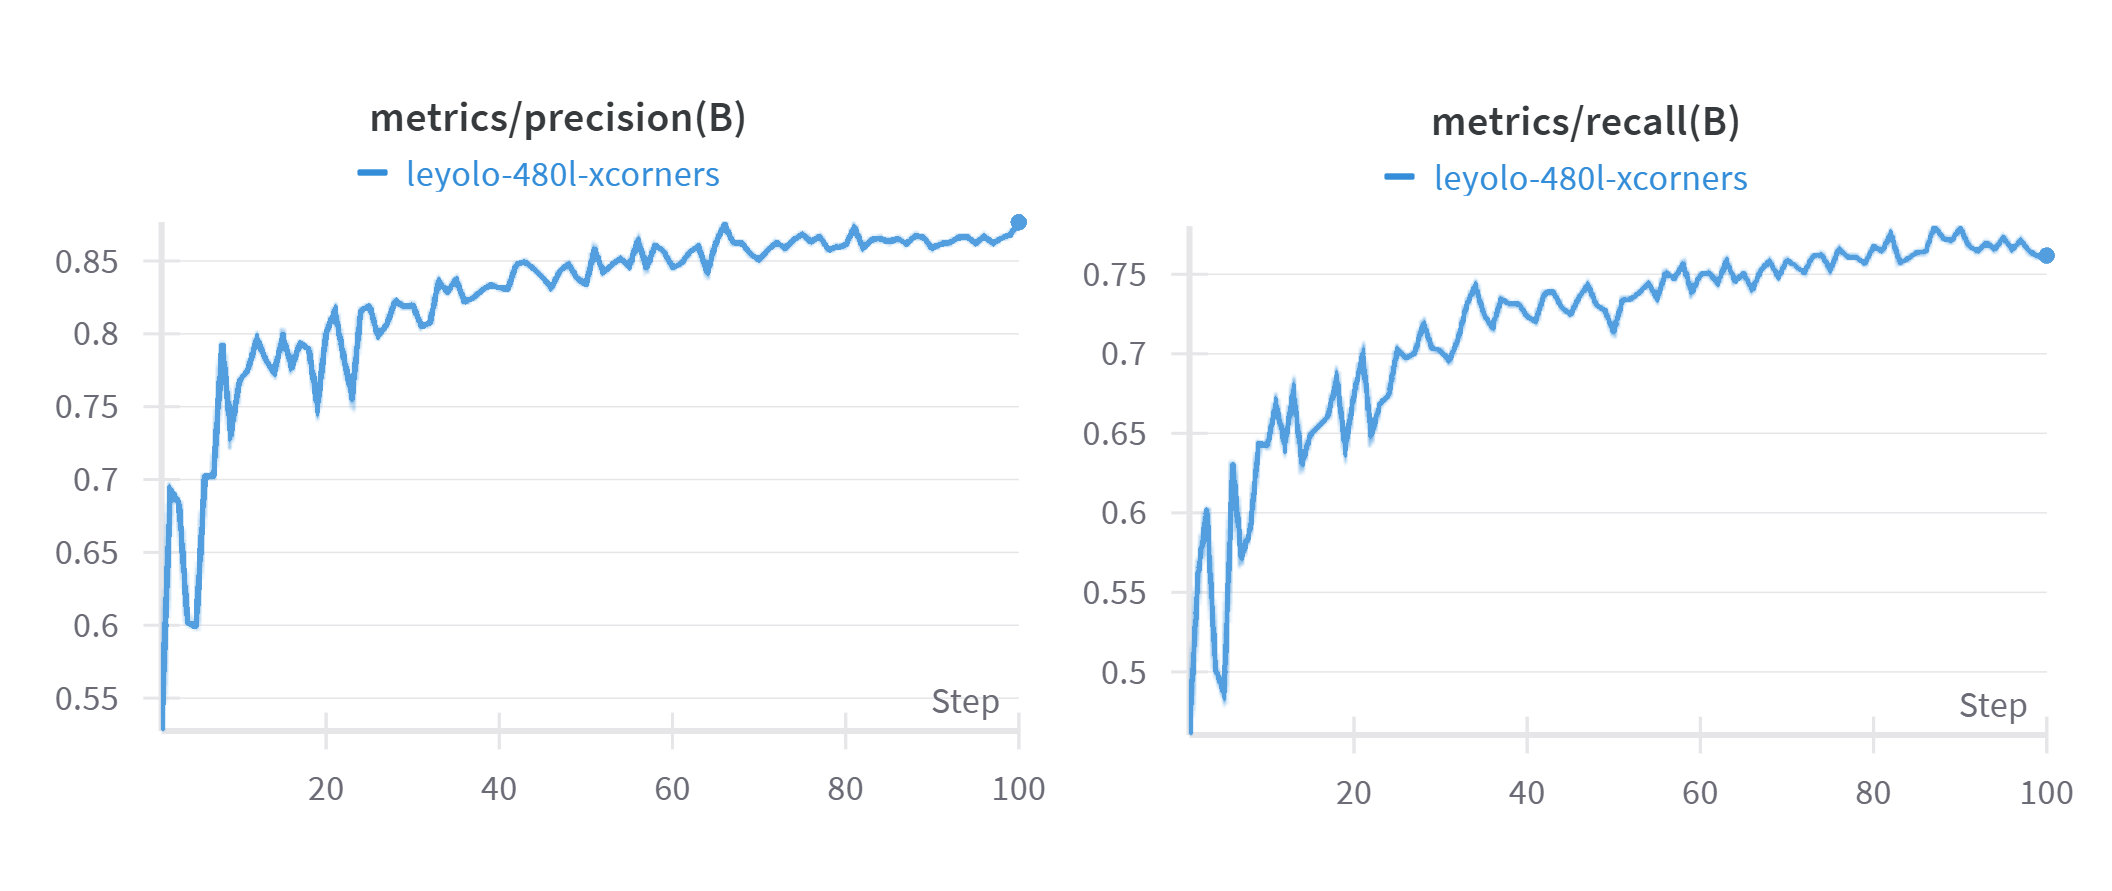
\includegraphics[width=\textwidth]{figures/results/machine-learning/xcorners-metrics.png}
\caption{Performance metrics for xcorners detection from ChessCam repository \cite{wandb:xcorner-detection}.}
\label{fig:chesscam-xcorners-metrics}
\end{figure}

\section{API}
To support continuous communication between the backend and frontend, the application establishes a WebSocket connection. This communication channel is used for transmitting move data as it is detected by the board recognition system. Unlike traditional \gls{http} requests, which operate on a request-response basis, WebSocket allows for continuous, two-way communication between the server and the client as described in \ref{subsubsec:websocket} \\

Once the application initiates a connection, the WebSocket remains open throughout the session. As new moves are identified on the physical board, the backend sends the corresponding move data as messages through the WebSocket. These messages are then received by the frontend, which updates the displayed move list and board state in real-time. \\

The WebSocket server also processes specific command messages to manage game state. For instance, a message labeled \texttt{RESET} prompts the frontend to clear the current move list, signaling the start of a new game, while simultaneously resetting the backend to prepare for a new tournament round. Conversely, a message labeled \texttt{INVALID} indicates an unrecognized or illegal move and does not result in any frontend updates. 


\section{Frontend}
\label{subsec:results-frontend}
The frontend of the application serves as the user interface. It includes a control panel for tournament organizers and a web application for spectators. The application's responsibility is to visualize the chessboard and display ongoing moves. The frontend communicates with the backend via WebSocket to ensure real-time updates. \\

The control panel is a standalone administrative interface used by tournament organizers to configure and manage the tournament setup. It allows the organizer to select the number of cameras, initiate the tournament, and reset boards between rounds, as shown in Figure~\ref{fig:control-panel}. This interface ensures the centralized management of tournament operations. \\

\begin{figure}[h!] \centering 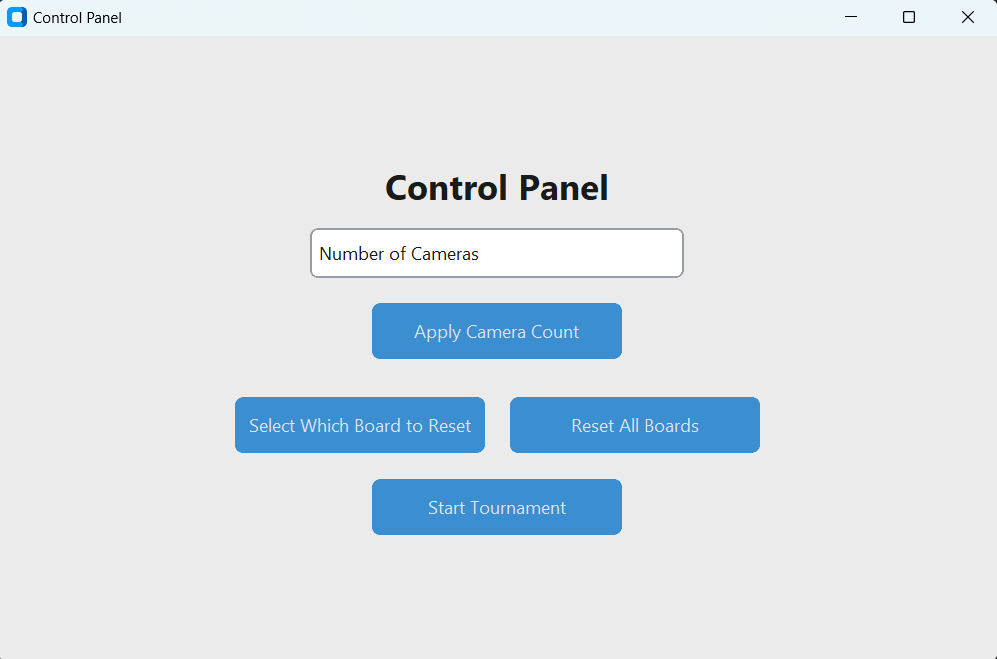
\includegraphics[width=0.75\linewidth]{figures/results/frontend/control-panel/control-panel.png} \caption[Control panel for tournament organizers]{The control panel used by the tournament organizers.}\label{fig:control-panel} \end{figure}

Once the application is launched, the accompanying web application becomes accessible to spectators. It is designed to allow viewers to follow the tournament across a range of devices. Spectators can navigate between views, observe live games, and explore additional information about the system. Built as a responsive interface, it adapts to both desktop and mobile screens to ensure accessibility and usability. \\

The landing page is The Tournament View. The Tournament View presents an overview of all ongoing games. Each entry shows the board number, the players' names and ratings, and a link to follow the game live, as shown in Figure~\ref{fig:tournament-view-mocked}. \\

\begin{figure}[h!] \centering \fbox{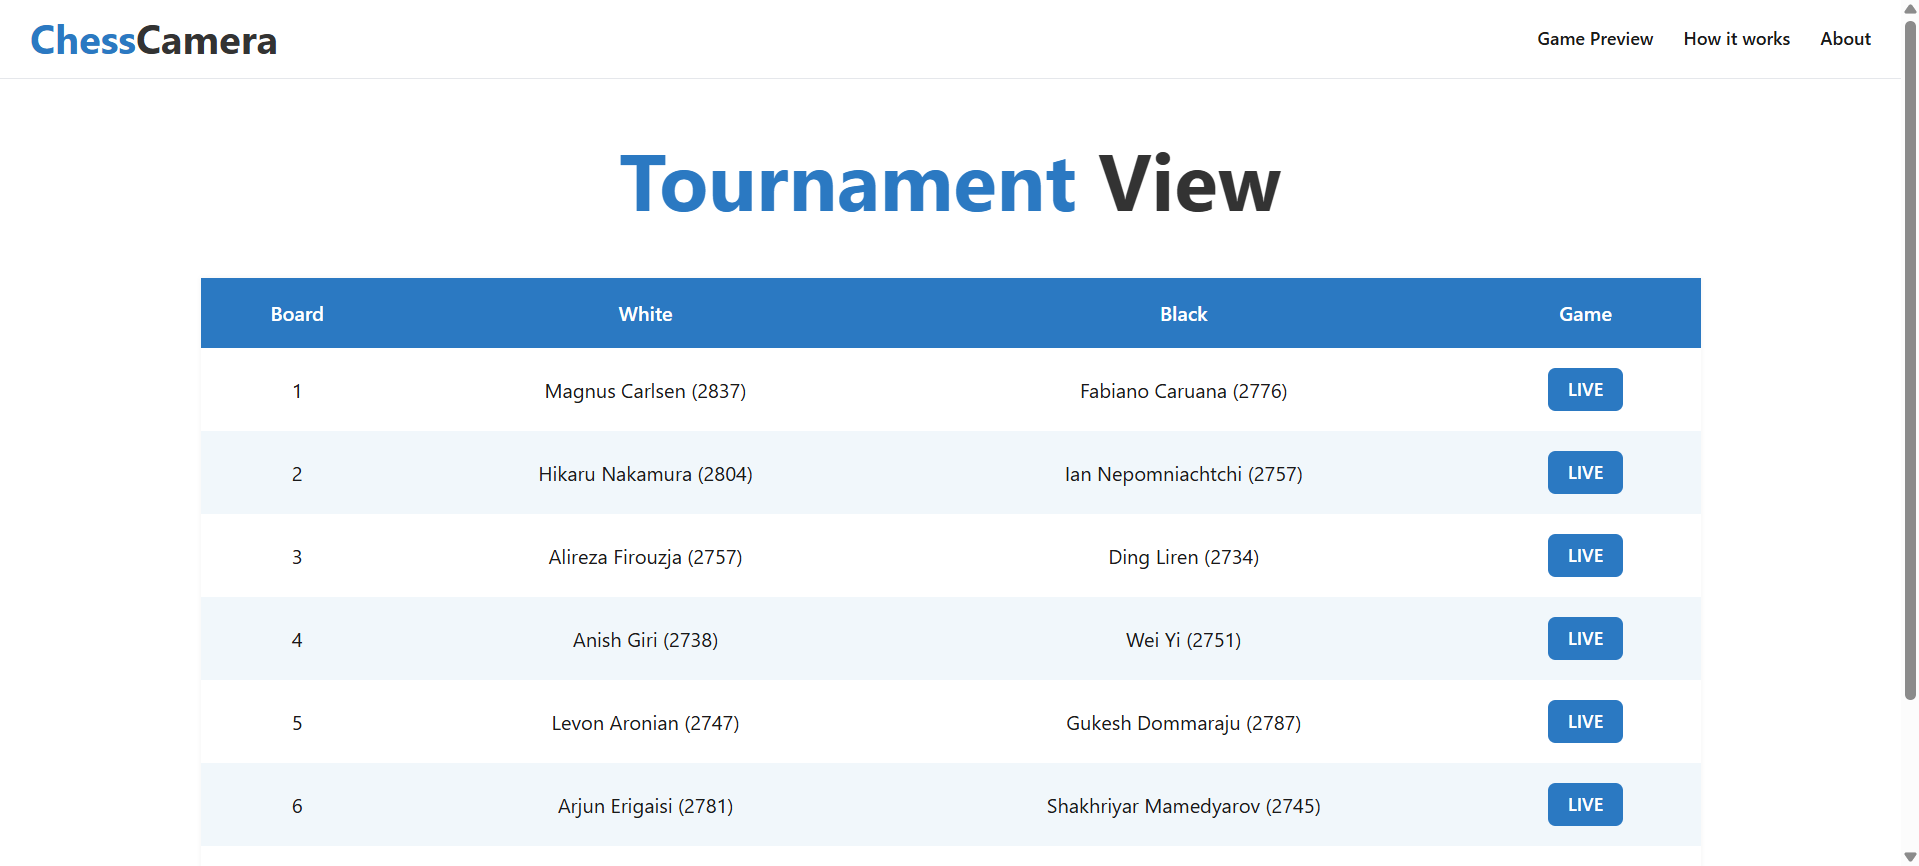
\includegraphics[width=0.75\linewidth]{figures/results/frontend/tournament-view/mocked.png}}\caption[Display of tournament]{A mocked demonstration of a tournament display.}\label{fig:tournament-view-mocked} \end{figure}

Another page is the Game Preview, which displays miniature boards for multiple games. This view provides an overview of all active games, allowing users to quickly identify and select any match for detailed viewing, as shown in Figure~\ref{fig:game-preview}. It offers an efficient way to stay updated on several games at once. \\

\begin{figure}[h!] \centering \fbox{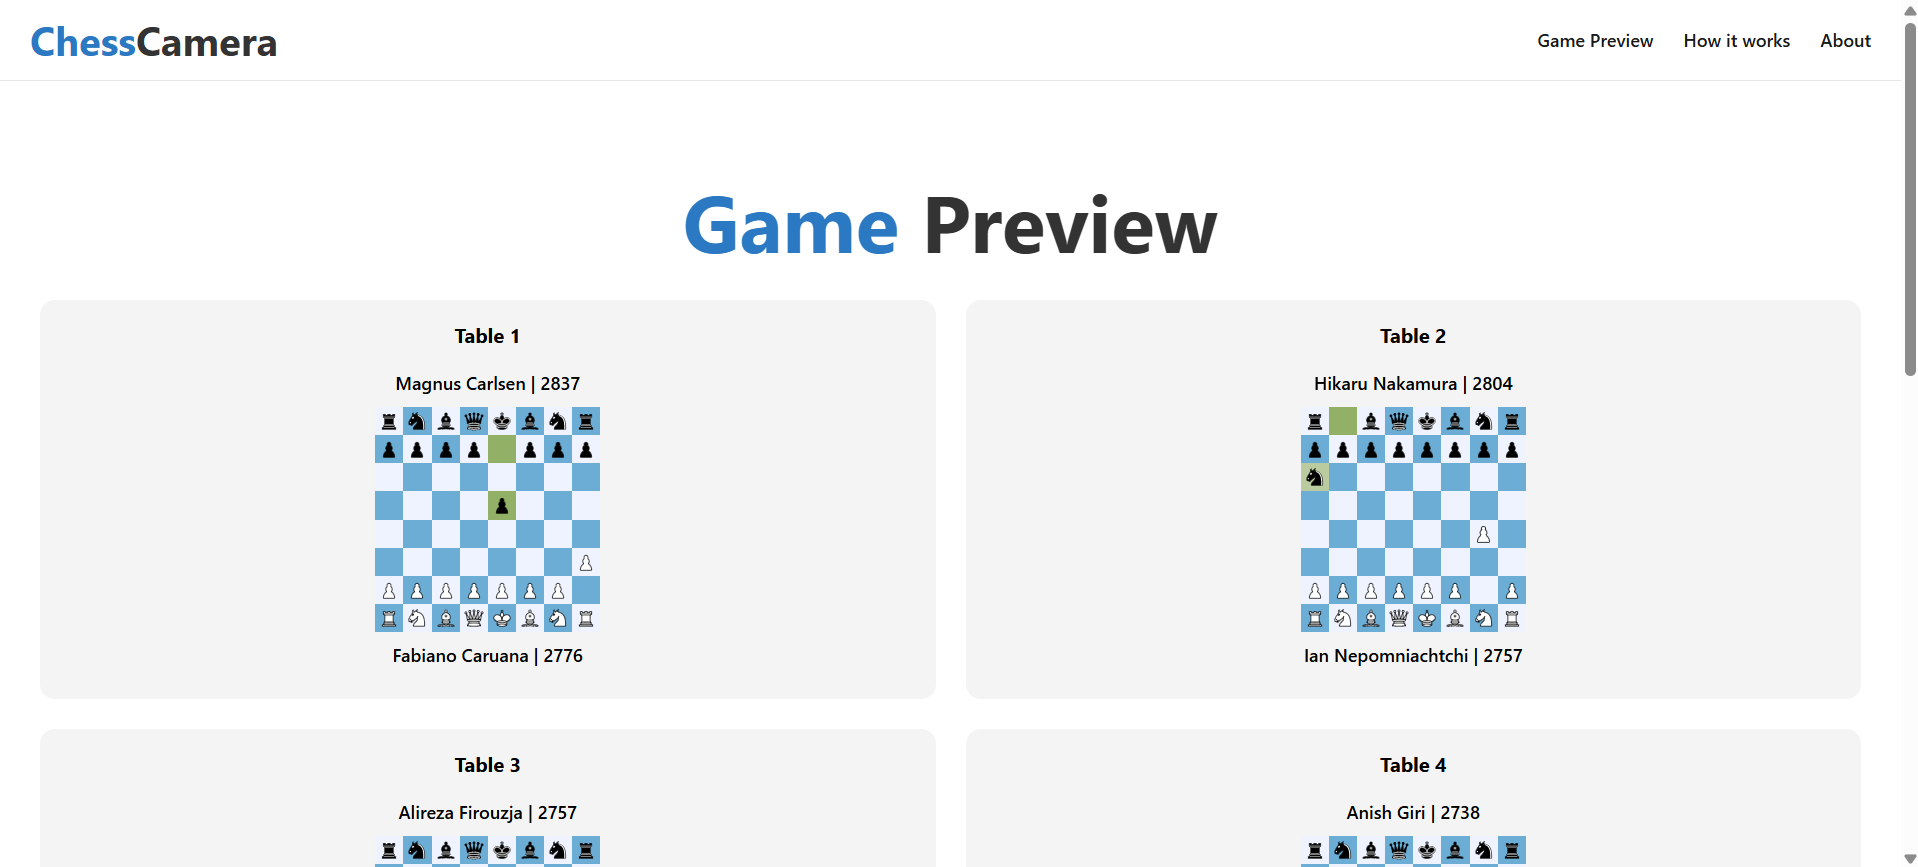
\includegraphics[width=0.75\linewidth]{figures/results/frontend/game-preview/desktop.png}}\caption[Preview of active games]{A mocked demonstration of a game preview page.}\label{fig:game-preview} \end{figure}

One of the main pages in the web application is the The Board View. The Board View presents a detailed view of a single game. It features a digital chessboard, a list of moves played, a live camera feed, and an evaluation bar, as shown in Figure~\ref{fig:download-pgn}. The elements update in real-time, creating an engaging experience for users. On the Board View page, users can download the \gls{pgn} file of the current game via a dedicated button, which saves the file locally. The board view is shown in Figure~\ref{fig:download-pgn}. \\

\begin{figure}[h!] \centering \fbox{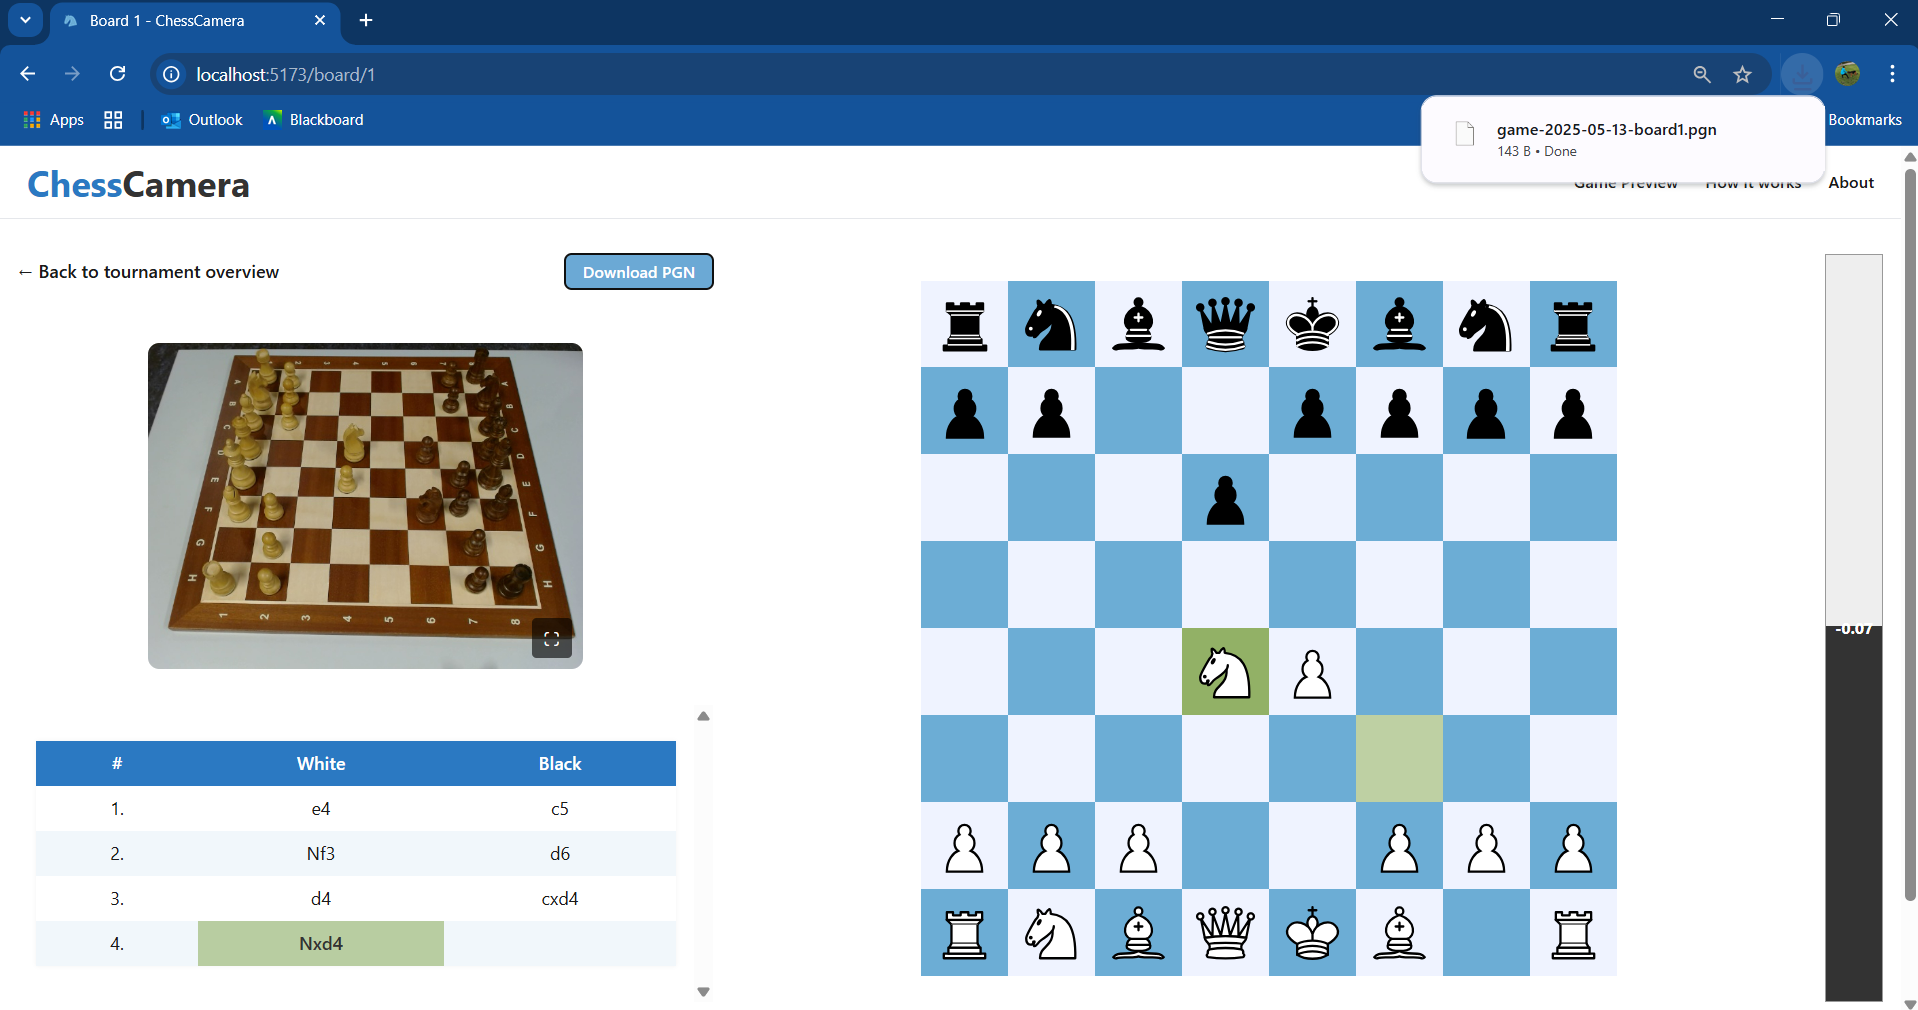
\includegraphics[width=0.75\linewidth]{figures/results/frontend/download-pgn/download-pgn.png}}\caption[Preview of downloading a PGN file]{A demonstration of downloading a PGN file to a specific game}\label{fig:download-pgn} \end{figure}

The downloaded file includes a header with key information such as the tournament name, date, and player names, followed by the recorded moves. It also indicates whether the game is still in progress. When the game is completed, this field displays the result 1-0, 0-1, or $\frac{1}{2}$–$\frac{1}{2}$. Figure~\ref{fig:downloaded-pgn} shows an example of such a file. \\

\begin{figure}[h!] \centering \fbox{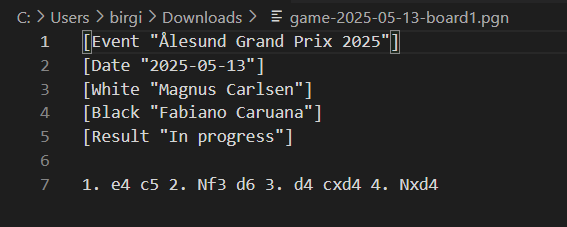
\includegraphics[width=0.75\linewidth]{figures/results/frontend/download-pgn/downloaded-pgn.png}}\caption[The downloaded PGN file]{The downloaded PGN file to a specific game, opened in a code editor}\label{fig:downloaded-pgn} \end{figure}

\section{Project Management}
\label{sec:results-project-management}
Although the project was initially structured according to the Scrum framework, its practical execution became more Scrum-inspired due to the absence of a dedicated Scrum Master and certain deviations from the full methodology. Each sprint began with a planning session in which tasks were selected from the product backlog based on priority and available team capacity. Sprint reviews were conducted at the end of each sprint to assess completed work and record outcomes. In addition, sprint retrospectives were held and documented, including reflections on workload distribution, communication challenges, and opportunities for process improvement. \\

Meeting routines were adapted according to team availability and project needs. Internal meetings were held as needed rather than on a fixed schedule, with most collaboration taking place informally during shared office hours. Nevertheless, short stand-up meetings were prioritized on a daily basis to maintain effective communication and ensure alignment. Biweekly meetings with the supervisor were consistently maintained, functioning as checkpoints for academic progress and clarification of requirements. Meetings with the product owner were arranged approximately once or twice per month and typically focused on feature validation, feedback, and adjustments. \\

GitHub was used consistently throughout the project for both task management and version control. Issues were linked to corresponding branches and categorized by type (e.g., feature, enhancement, documentation). All code changes were submitted via pull requests, and no changes were pushed directly to the main branch. Peer review was strictly enforced as part of the workflow, with every pull request reviewed by at least one team member before merging. \\

Tasks were assigned to individual team members and tracked using GitHub Issues. Issues were labeled and moved through the workflow stages: \textit{No Status}, \textit{To Do}, \textit{In Progress}, and \textit{Done}. This workflow was followed consistently for larger development tasks. However, some minor items, particularly quick fixes and small adjustments, were occasionally completed outside of the issue board during periods of intensive development, resulting in slightly reduced traceability for those changes.\\

In addition to manual code review, automated workflows were implemented using GitHub Actions to support continuous integration and reduce human error. One workflow was configured to run Python unit tests on every push, ensuring code stability throughout development. Another workflow was responsible for automatically updating LaTeX-based documentation by cloning the relevant repository and pushing changes after each update, as shown in Figure~\ref{fig:workflow-latex}. These pipelines contributed to improved reliability, automation of repetitive tasks, and early detection of breaking changes during development. \\

\begin{figure}[h!] \centering 
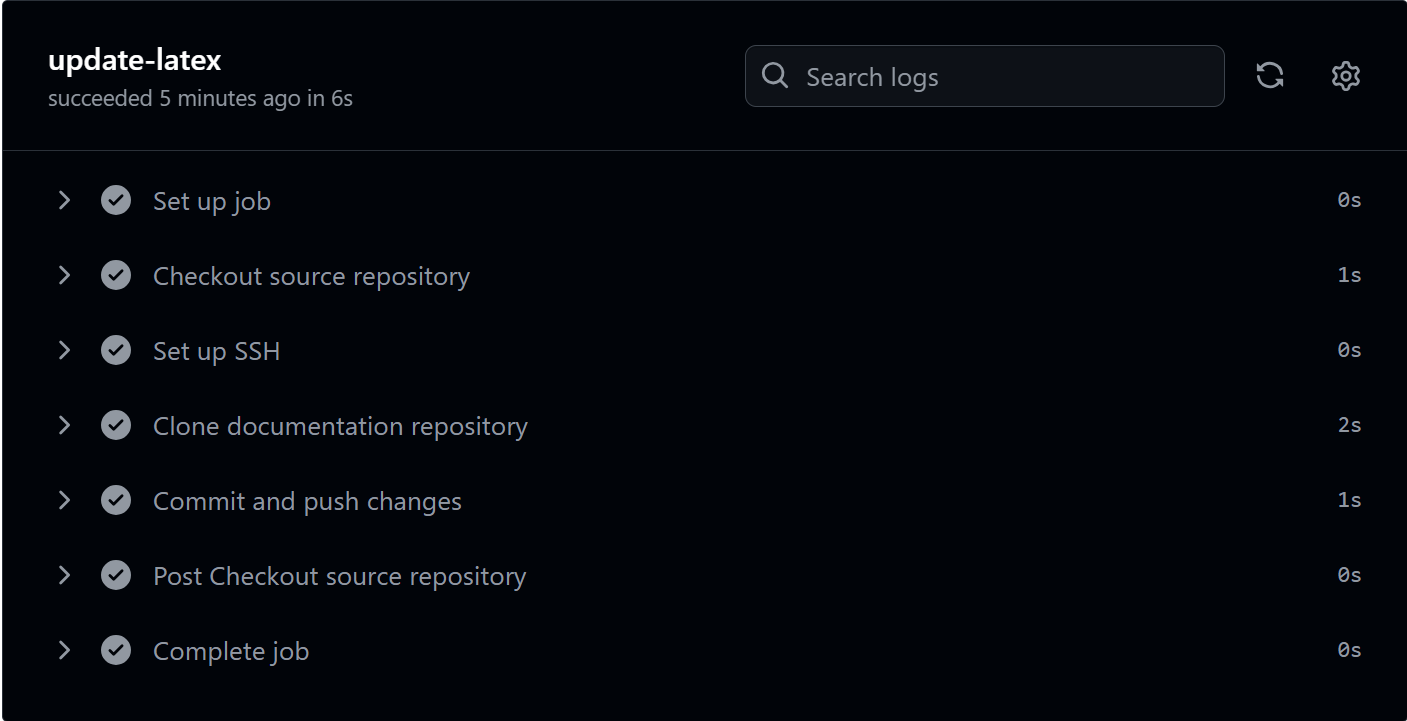
\includegraphics[width=0.75\linewidth]{figures/results/workflows/latex.png}\caption[Upload LaTeX workflow]{The workflow for update documentation with code}\label{fig:workflow-latex} \end{figure}

\section{Technical Achievements}

\subsection{Architecture Overview}
\label{subsec:diagrams}

To provide a comprehensive understanding of the system architecture and interaction flow, several \gls{uml} diagrams were created. These diagrams model different aspects of the live chess game digitization system, from component interactions and activity flow to user roles and use cases.

\subsubsection*{Sequence Diagram}
\label{subsubsec:sequence-diagram}

The sequence diagram, shown in Figure \ref{fig:sequence}, illustrates the chronological flow of interactions between the system components and external actors. It begins with the Admin initiating the game recording by setting up the camera, which captures and streams the board state to a local processing unit. This unit continuously detects and validates moves, updating the user interface accordingly. Users, from remote devices, can spectate the game in real-time or save it as a \gls{pgn} file. The diagram emphasizes the communication between hardware (camera and local machine) and the \gls{ui}, highlighting how physical chess games are digitized and broadcasted.

\newpage

\begin{figure}[h!]
    \centering
    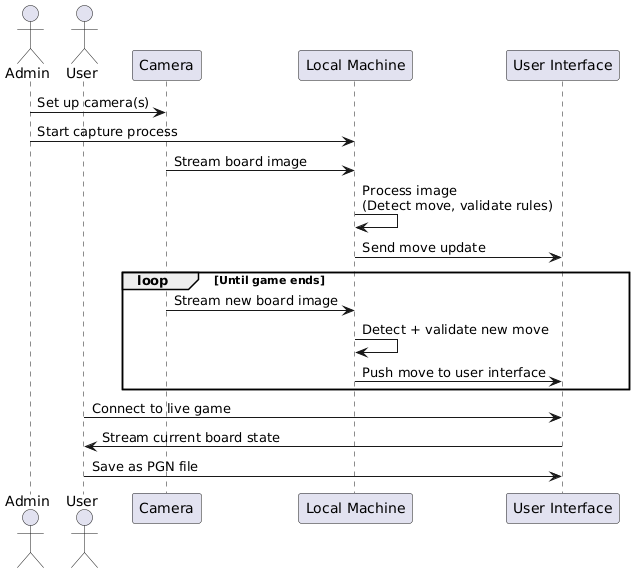
\includegraphics[width=\linewidth]{figures/results/uml/sequence.png}
    \caption[Sequence Diagram]{Sequence Diagram}
    \label{fig:sequence}
\end{figure}

\subsubsection*{Use-Case Diagram}
\label{subsubsec:use-case-diagram}

The use-case diagram, shown in Figure \ref{fig:use-case}, identifies the system’s main actors and the primaryfunctionalities they interact with. Admins are responsible for hardware setup and initiating the game recordingprocess. The system autonomously handles move detection, validation, and \gls{ui} updates. Users, on the otherhand, access the game remotely to spectate or download \gls{pgn} files. This diagram provides a clear overview ofwho interacts with the system and what capabilities are exposed, forming the basis for understanding systemrequirements and user expectations.

\begin{figure}[h!]
    \centering
    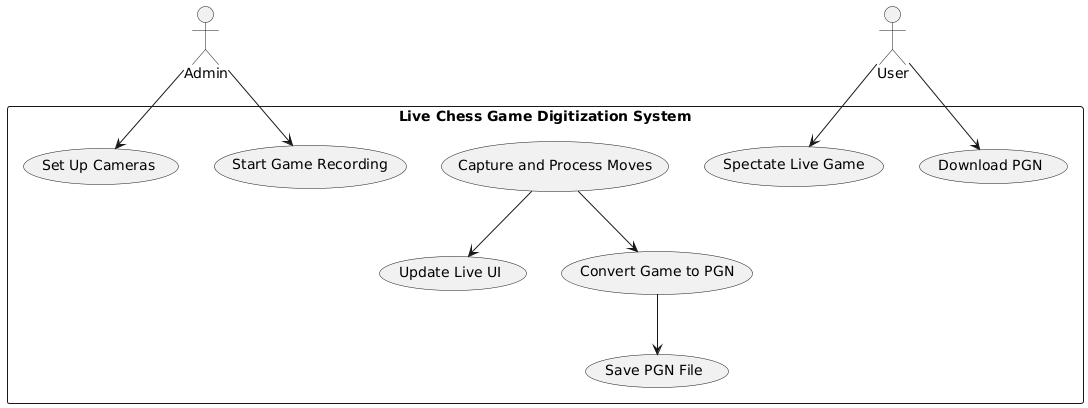
\includegraphics[width=\linewidth]{figures/results/uml/use-case.png}
    \caption{Use-Case Diagram}
    \label{fig:use-case}
\end{figure}  

\begin{figure}[h!]
    \subsubsection*{Activity Diagram}
    \label{subsubsec:activity-diagram}
    
    \centering
    \begin{minipage}[t]{0.5\textwidth}
        \vspace{0pt}
        The activity diagram, shown in Figure \ref{fig:activity}, provides a high-level overview of the operational workflow during a chess game session. It models the continuous loop of capturing board states, detecting and validating moves, and updating the game state until the game ends. If a move is invalid, the system flags it but does not terminate the session. Once the game concludes, it is converted into a standard \gls{pgn} format. This diagram emphasizes the logical flow and decision-making process, reflecting the system’s role in automating and maintaining the integrity of live digitization.
    \end{minipage}
    \hfill
    \begin{minipage}[t]{0.45\textwidth}
        \vspace{0pt}
        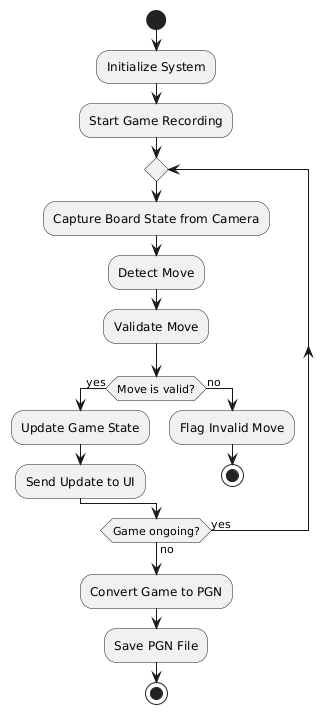
\includegraphics[width=\linewidth]{figures/results/uml/activity-2.png}
        \caption[Activity Diagram]{Activity Diagram}
        \label{fig:activity}
    \end{minipage}
\end{figure}

\newpage

\subsubsection*{Class Diagram}

The most widely use UML diagram is the class diagram. It is the building block of all object oriented software systems. We use class diagrams to depict the static structure of a system by showing system's classes, their methods and attributes. Class diagrams also help us identify relationship between different classes or objects.

\begin{figure}[h!]
    \centering
    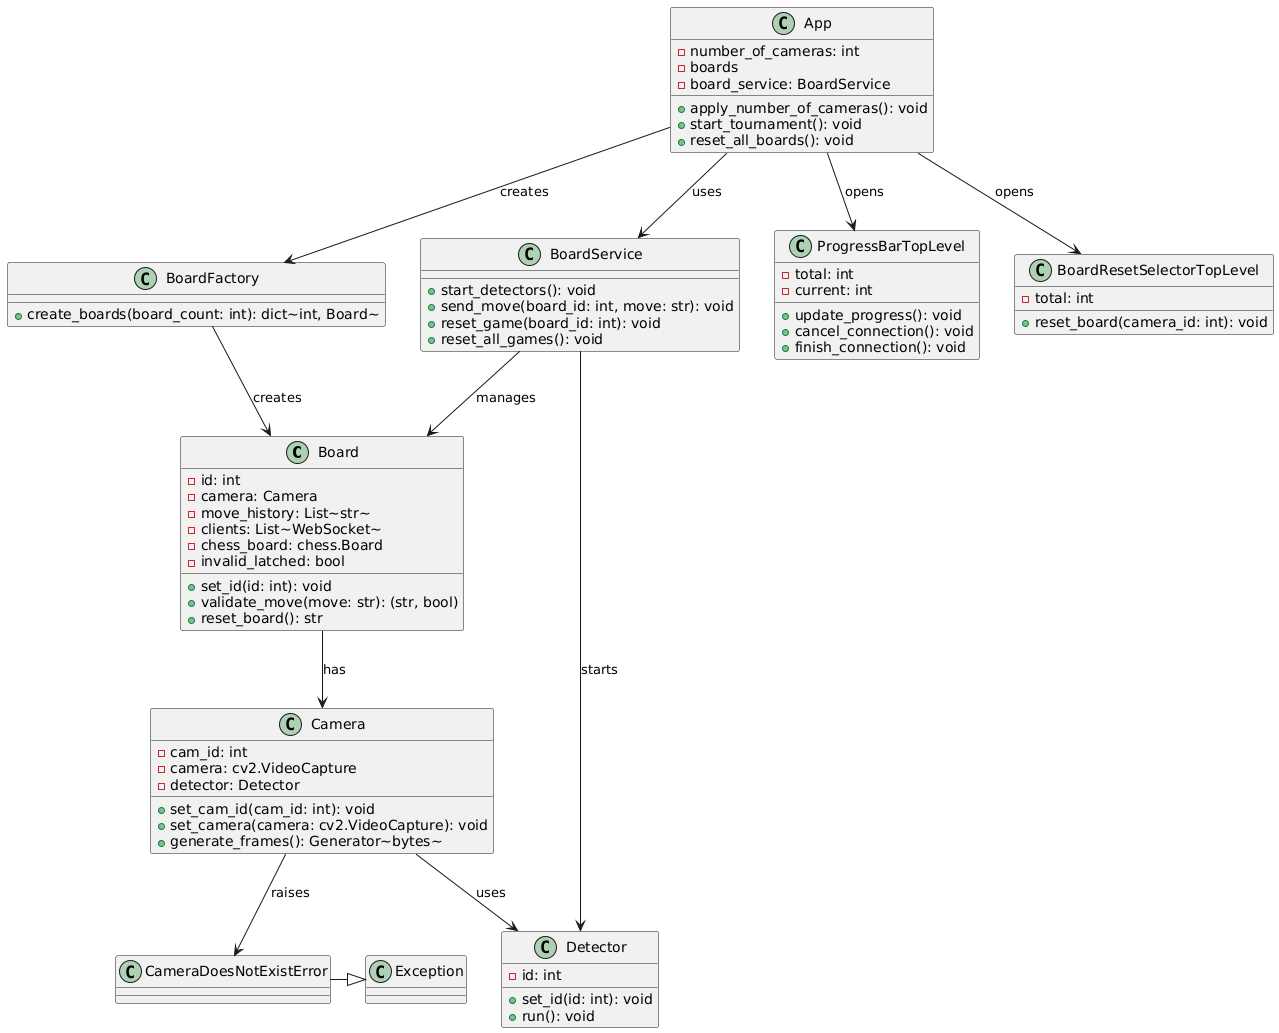
\includegraphics[width=\linewidth]{figures/results//uml/class.png}
    \caption{Class Diagram}
    \label{fig:class}
\end{figure}

\begin{figure}[h!]
    \subsubsection*{State Machine Diagram}
    \label{subsubsec:state-machine-diagram}

    \centering
    \begin{minipage}[t]{0.45\textwidth}
        A state diagram is used to represent the condition of the system or part of the system at finite instances of time. It’s a behavioral diagram and it represents the behavior using finite state transitions.

        \begin{itemize}
            \item State diagrams are also referred to as State machines and State-chart Diagrams
            \item These terms are often used interchangeably. So simply, a state diagram is used to model the dynamic behavior of a class in response to time and changing external stimuli.
        \end{itemize}
    \end{minipage}
    \hfill
    \begin{minipage}[t]{0.5\textwidth}
        \vspace{0pt}
        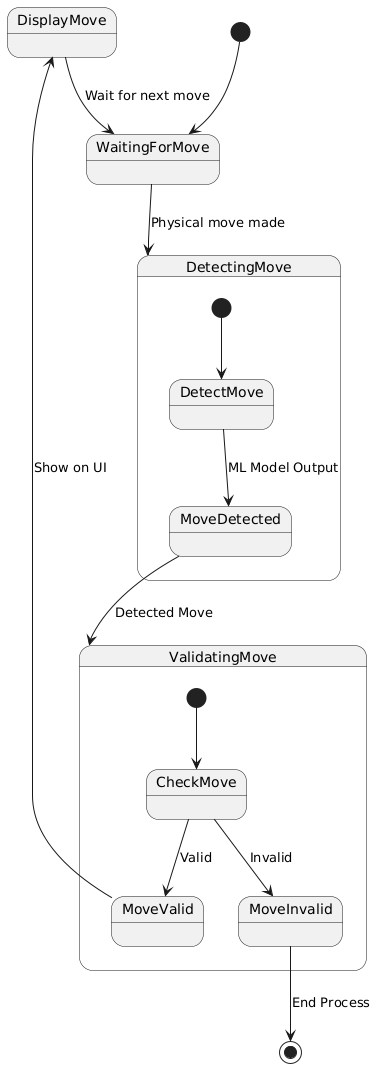
\includegraphics[width=\linewidth]{figures/results/uml/state-machine.png}
        \caption[State Machine Diagram]{State Machine Diagram}
        \label{fig:state-machine}
    \end{minipage}
\end{figure}

\newpage

\newpage

\subsubsection*{Package Diagram}

We use Package Diagrams to depict how packages and their elements have been organized. A package diagram simply shows us the dependencies between different packages and internal composition of packages.

\begin{itemize}
    \item Packages help us to organise UML diagrams into meaningful groups and make the diagram easy to understand.
    \item They are primarily used to organise class and use case diagrams.
\end{itemize}

\begin{figure}[h!]
    \centering
    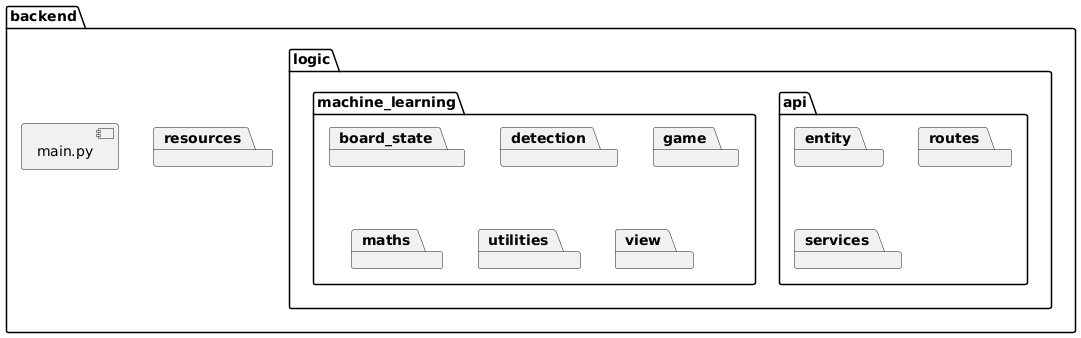
\includegraphics[width=\linewidth]{figures/results//uml/package-backend.png}
    \caption{Package Diagram for Backend}
    \label{fig:package-backend}
\end{figure}

\begin{figure}[h!]
    \centering
    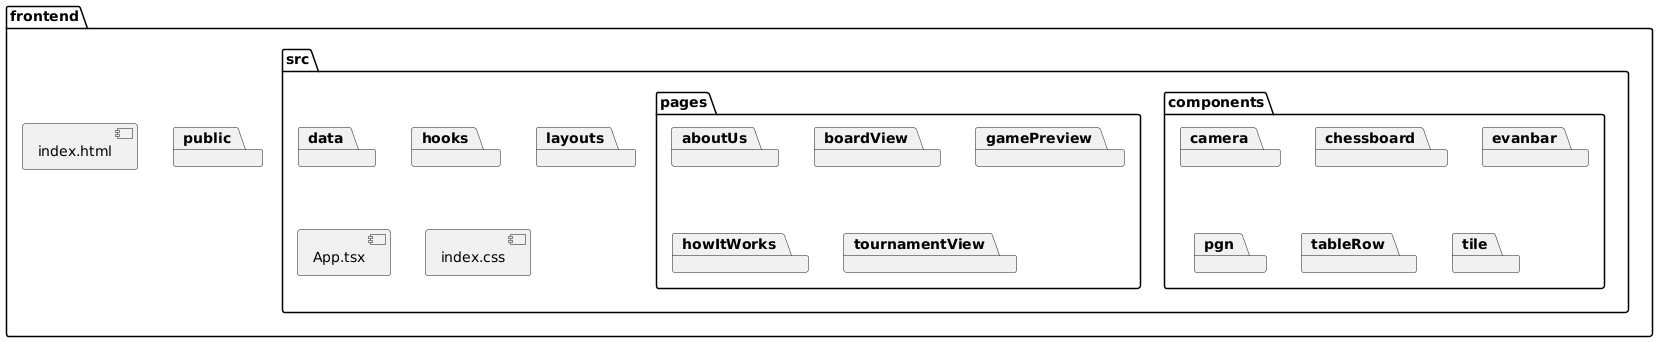
\includegraphics[width=\linewidth]{figures/results//uml/package-frontend.png}
    \caption{Package Diagram for Frontend}
    \label{fig:package-frontend}
\end{figure}
\subsection{Manual Testing}

\subsection{Machine Learning Model}
\label{machine-learning-test}

As described in Section~\ref{subsec:model-testing}, the model was evaluated using 100 games. Table~\ref{tab:accuracy-total} presents the overall move detection accuracy, both in total and broken down by piece type and color. The model achieved an overall accuracy of 90.6\%, successfully detecting 936 out of 1033 moves. Pawns had the highest detection rates, with over 98\% accuracy for both colors. In contrast, the model struggled particularly with black rooks with only 23.8\% accuracy.

\begin{table}[htbp]
\centering
\caption{Move detection accuracy in total}
\label{tab:accuracy-total}
\begin{tabular}{lccc}
\toprule
\textbf{Category} & \textbf{OTB Moves} & \textbf{Successful Moves} & \textbf{Accuracy (\%)} \\
\midrule
\textbf{White Pieces} & & & \\
\hspace{1em}Pawn  & 244 & 242 & 99.2\% \\
\hspace{1em}Knight & 128 & 117 & 91.4\% \\
\hspace{1em}Bishop & 74  & 54  & 73.0\% \\
\hspace{1em}Rook   & 29  & 25  & 86.2\% \\
\hspace{1em}Queen  & 42  & 40  & 95.2\% \\
\hspace{1em}King   & 16  & 8   & 50.0\% \\
\midrule
\textbf{Black Pieces} & & & \\
\hspace{1em}Pawn  & 247 & 243 & 98.4\% \\
\hspace{1em}Knight & 78  & 75  & 96.2\% \\
\hspace{1em}Bishop & 65  & 47  & 72.3\% \\
\hspace{1em}Rook   & 21  & 5   & 23.8\% \\
\hspace{1em}Queen  & 84  & 76  & 90.5\% \\
\hspace{1em}King   & 5   & 4   & 80.0\% \\
\midrule
\textbf{Total} & 1033 & 936 & 90.6\% \\
\bottomrule
\end{tabular}
\end{table}


Table~\ref{tab:board-type-accuracy} compares the success rates between the two physical board types used during testing. The wooden board slightly outperformed the plastic board, with a 91.2\% success rate compared to 89.9\%. This marginal difference may indicate a slightly more stable detection environment on the wooden surface. \\


\begin{table}[htbp]
\centering
\caption{Summary of Total Moves and Success Rate by Board Type}
\label{tab:board-type-accuracy}
\begin{tabular}{lccc}
\toprule
\textbf{Board Type} & \textbf{Total Moves} & \textbf{Total Successful Moves} & \textbf{Success Rate (\%)} \\
\midrule
Plastic & 475 & 427 & 89.9\% \\
Wooden  & 558 & 509 & 91.2\% \\
\bottomrule
\end{tabular}
\end{table}


Figure~\ref{fig:move-failures} shows the number of failed games (i.e., games where detection failed) grouped by the move number at which failure occurred. Bars are color-coded by board type. The majority of failures occurred within the first five moves, particularly at moves 2, 4, and 5. This trend suggests that the early game presents the greatest challenge for detection, potentially due to rapid development or ambiguity in piece positions. Notably, failures after move 9 were rare. \\


\begin{figure}[htbp]
\centering
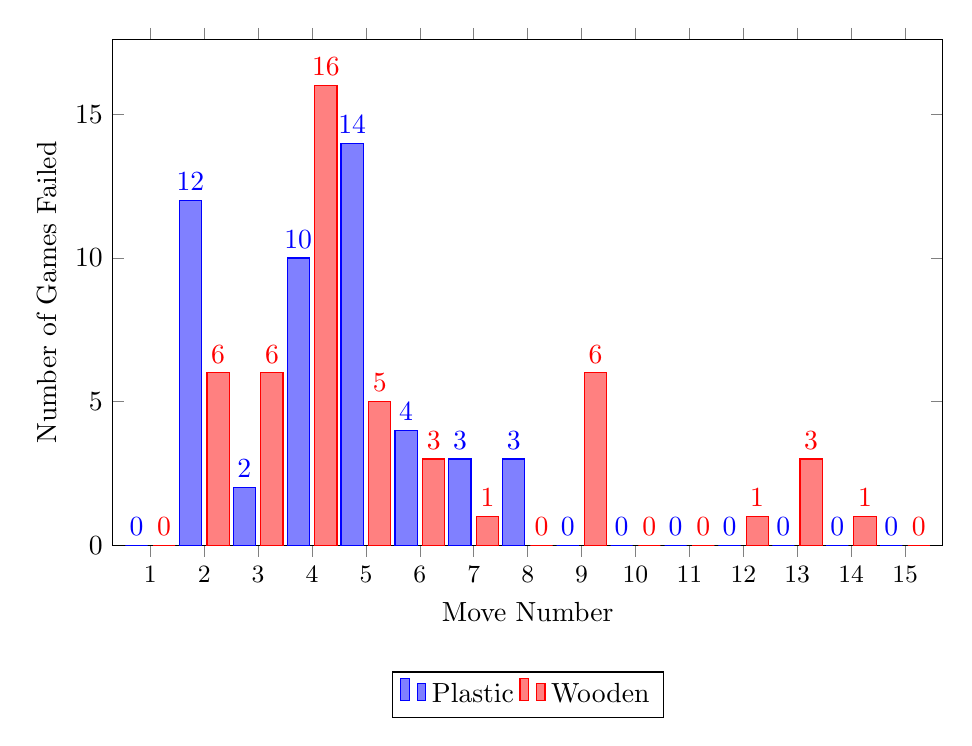
\begin{tikzpicture}
\begin{axis}[
    ybar,
    bar width=8pt,
    width=\textwidth,
    height=8cm,
    enlarge x limits=0.05,
    ymin=0,
    ylabel={Number of Games Failed},
    xlabel={Move Number},
    xtick={1,...,15},
    xticklabels={1,2,3,4,5,6,7,8,9,10,11,12,13,14,15},
    x tick label style={rotate=0, anchor=north, font=\small},
    legend style={at={(0.5,-0.25)}, anchor=north, legend columns=-1},
    nodes near coords,
    symbolic x coords={1,2,3,4,5,6,7,8,9,10,11,12,13,14,15},
    xticklabel style={font=\small},
]
\addplot+[style={fill=blue!50}] coordinates {
    (1,0) (2,12) (3,2) (4,10) (5,14) (6,4) (7,3) (8,3) (9,0)
    (10,0) (11,0) (12,0) (13,0) (14,0) (15,0)
};
\addplot+[style={fill=red!50}] coordinates {
    (1,0) (2,6) (3,6) (4,16) (5,5) (6,3) (7,1) (8,0) (9,6)
    (10,0) (11,0) (12,1) (13,3) (14,1) (15,0)
};
\legend{Plastic, Wooden}
\end{axis}
\end{tikzpicture}
\caption{Number of failed games per move number across plastic and wooden boards.}
\label{fig:move-failures}
\end{figure}


Table~\ref{tab:different-errors} categorizes the types of detection failures for each board type. The majority of failures were due to a complete lack of detection within the allotted time window. Incorrect detections (the model detecting a move but interpreting it wrongly) were less frequent but more common on the wooden board, accounting for 8 out of 48 failures, compared to just 1 on the plastic board.  \\

\begin{table}[htbp]
\centering
\caption{Frequencies of Different Detection Errors}
\label{tab:different-errors}
\begin{tabular}{lccc}
\toprule
\textbf{Board Type} & \textbf{Total Failures} & \textbf{No Detection} & \textbf{Incorrect Detection} \\
\midrule
Plastic & 48 & 47 & 1 \\
Wooden & 48 & 40 & 8 \\
\midrule
\textbf{Total} & 96 & 87 & 9 \\
\bottomrule
\end{tabular}
\end{table}

For a detailed breakdown of the chess games, including the sequences of moves, failure points, and detection statistics for each board type, see Appendix FILL IN.

\subsection{Wireframe}
\label{subsec:wireframe-results}

A total of eight individuals participated in the wireframe usability test, excluding project developers and stakeholders. While the sample size was limited, participants were intentionally selected to represent a broad range of ages, technical backgrounds, and familiarity with chess. \\

Overall, the feedback was generally positive. Participants were asked to rate their satisfaction on a 1–5 Likert scale. Figure \ref{fig:wireframe-test-results} shows the distribution of the ratings. The average scores from the feedback form were as follows:

\begin{itemize}
    \item The \textbf{overall user experience} received an average rating of \textbf{4.63} out of 5.
    \item The \textbf{Tournament View page} received the highest average rating of \textbf{4.75}.
    \item The \textbf{Board View page} received a slightly lower average rating of \textbf{4.38}.
\end{itemize}

Participants commented that the interface was easy to navigate and that the layout felt intuitive. The Tournament View, in particular, was praised for its clarity and structure. Several testers without prior experience using chess-related software indicated that the interface felt approachable and visually clear. \\

However, participants also suggested a few areas for improvement:

\begin{itemize}
    \item Adding a full-screen function for the video feed.
    \item Enhancing the visual design of some UI elements for improved aesthetics.
    \item Supporting multiple languages for users who do not speak English.
\end{itemize}

While these findings are based on a small participant group, they offer early indications that the interface is both accessible and functional for a wide range of users. These insights will guide further development and refinement of the user interface.

\begin{figure}[htbp]
\centering
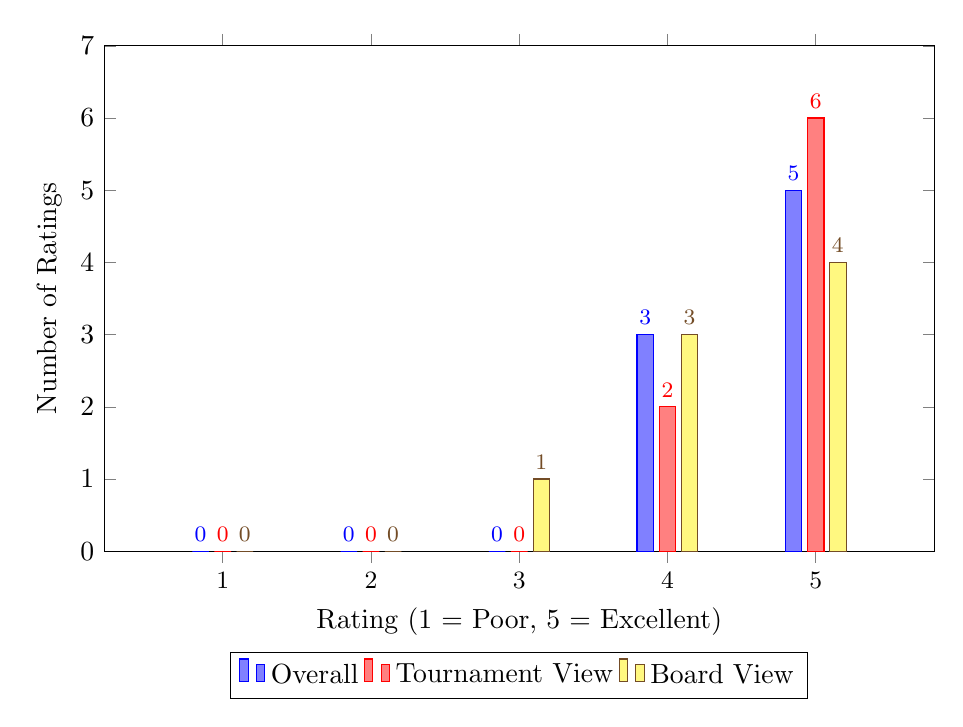
\begin{tikzpicture}
\begin{axis}[
    ybar,
    bar width=6pt,
    width=\textwidth,
    height=8cm,
    enlarge x limits=0.2,
    ymin=0,
    ymax=7,
    ylabel={Number of Ratings},
    xlabel={Rating (1 = Poor, 5 = Excellent)},
    symbolic x coords={1,2,3,4,5},
    xtick=data,
    x tick label style={rotate=0, anchor=north, font=\small},
    legend style={
        at={(0.5,-0.2)},
        anchor=north,
        legend columns=3
    },
    nodes near coords,
    nodes near coords style={font=\footnotesize},
    every node near coord/.append style={
        /pgf/number format/.cd,
        fixed,
        precision=0,
        /tikz/ifthenelse/.code={
            \ifnum\pgfplotspointmeta=0
                \pgfkeys{/pgfplots/disable node}
            \fi
        }
    }
]
\addplot+[style={fill=blue!50}] coordinates {
    (1,0) (2,0) (3,0) (4,3) (5,5)
};
\addplot+[style={fill=red!50}] coordinates {
    (1,0) (2,0) (3,0) (4,2) (5,6)
};
\addplot+[style={fill=yellow!50}] coordinates {
    (1,0) (2,0) (3,1) (4,3) (5,4)
};
\legend{Overall, Tournament View, Board View}
\end{axis}
\end{tikzpicture}
\caption{Distribution of satisfaction ratings from participants across different interface views.}
\label{fig:wireframe-test-results}
\end{figure}



\subsection{Color Palette}
\label{subsec:results-color-palette}
Voting revealed a mix of preferences: some participants favored the light mode from palette \#08 and the dark mode from palette \#07, while others selected the board design from palette \#05 or the move-highlighting style from palette \#14. \\

Rather than selecting a single predefined palette, the final color scheme was assembled by combining the most highly rated elements across the top-voted variations, yielding a more tailored, user-informed visual design. Figure \ref{fig:color-palette-results} shows the distribution of votes across all tested palettes; the full set of prototypes appears in Appendix \ref{app:color-palettes}.

\begin{figure}[htbp]
\centering
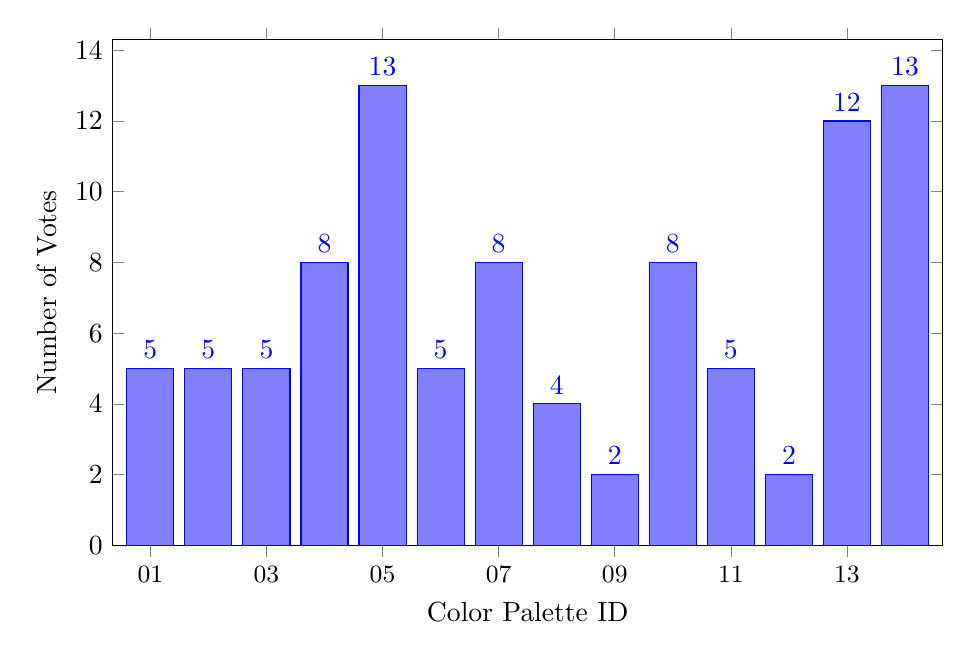
\begin{tikzpicture}
\begin{axis}[
    ybar,
    bar width=17pt,
    width=\textwidth,
    height=8cm,
    enlarge x limits=0.05,
    ymin=0,
    ylabel={Number of Votes},
    xlabel={Color Palette ID},
    xticklabels={01,02,03,04,05,06,07,08,09,10,11,12,13,14},
    x tick label style={rotate=0, anchor=north, font=\small},
    nodes near coords,
    symbolic x coords={01,02,03,04,05,06,07,08,09,10,11,12,13,14},
    xticklabel style={font=\small},
]
\addplot+[style={fill=blue!50}] coordinates {
    (01, 5) (02, 5) (03, 5) (04, 8) (05, 13) (06, 5) (07, 8) (08, 4) (09, 2) (10, 8) (11, 5) (12, 2) (13, 12) (14, 13)
};
\end{axis}
\end{tikzpicture}
\caption{Distribution of Votes Across Different Color Palettes}
\label{fig:color-palette-results}
\end{figure}